% Created by tikzDevice version 0.10.1 on 2018-06-30 02:11:43
% !TEX encoding = UTF-8 Unicode
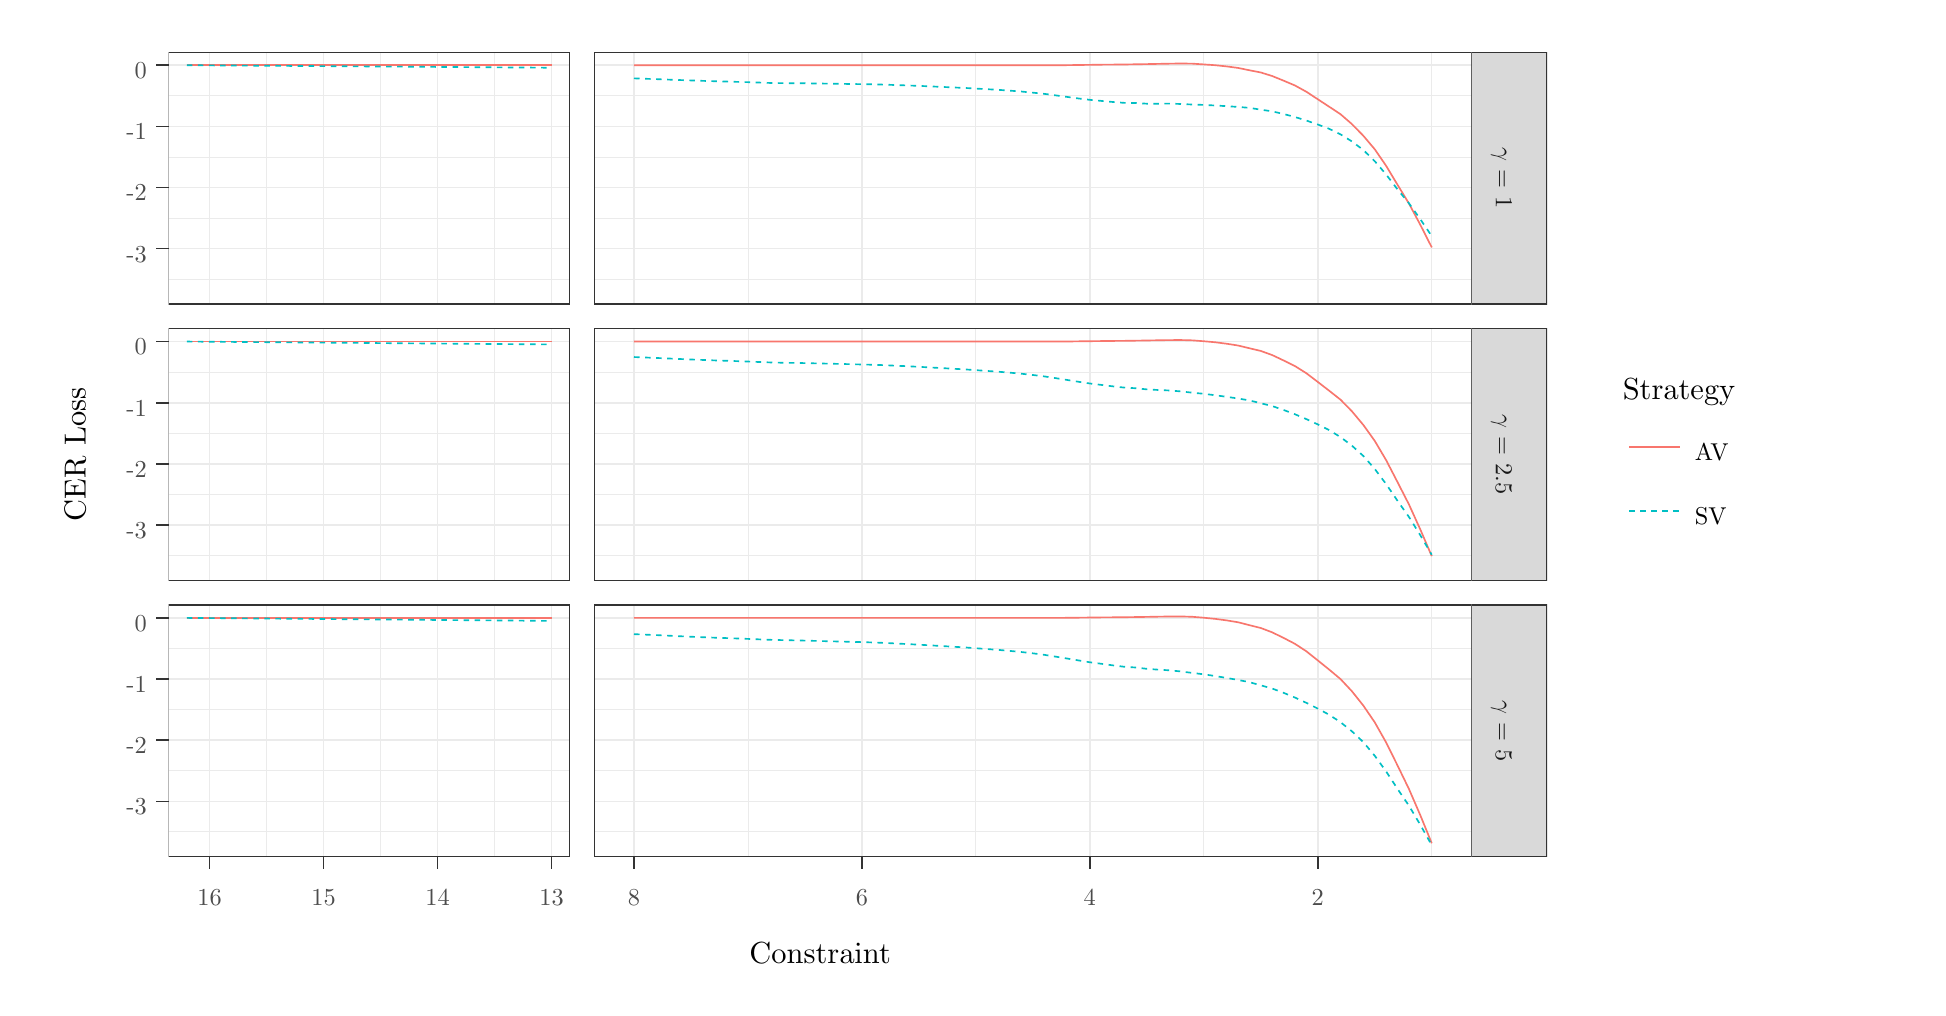
\begin{tikzpicture}[x=1.6pt,y=1.6pt]
\definecolor{fillColor}{RGB}{255,255,255}
\path[use as bounding box,fill=fillColor,fill opacity=0.00] (0,0) rectangle (426.79,216.81);
\begin{scope}
\path[clip] (  0.00,  0.00) rectangle (426.79,216.81);
\definecolor{drawColor}{RGB}{255,255,255}
\definecolor{fillColor}{RGB}{255,255,255}

\path[draw=drawColor,line width= 0.6pt,line join=round,line cap=round,fill=fillColor] (  0.00,  0.00) rectangle (426.79,216.81);
\end{scope}
\begin{scope}
\path[clip] ( 31.83,154.40) rectangle (122.43,211.31);
\definecolor{fillColor}{RGB}{255,255,255}

\path[fill=fillColor] ( 31.83,154.40) rectangle (122.43,211.31);
\definecolor{drawColor}{gray}{0.92}

\path[draw=drawColor,line width= 0.3pt,line join=round] ( 31.83,160.00) --
	(122.43,160.00);

\path[draw=drawColor,line width= 0.3pt,line join=round] ( 31.83,173.80) --
	(122.43,173.80);

\path[draw=drawColor,line width= 0.3pt,line join=round] ( 31.83,187.61) --
	(122.43,187.61);

\path[draw=drawColor,line width= 0.3pt,line join=round] ( 31.83,201.42) --
	(122.43,201.42);

\path[draw=drawColor,line width= 0.3pt,line join=round] (105.44,154.40) --
	(105.44,211.31);

\path[draw=drawColor,line width= 0.3pt,line join=round] ( 79.70,154.40) --
	( 79.70,211.31);

\path[draw=drawColor,line width= 0.3pt,line join=round] ( 53.96,154.40) --
	( 53.96,211.31);

\path[draw=drawColor,line width= 0.6pt,line join=round] ( 31.83,166.90) --
	(122.43,166.90);

\path[draw=drawColor,line width= 0.6pt,line join=round] ( 31.83,180.71) --
	(122.43,180.71);

\path[draw=drawColor,line width= 0.6pt,line join=round] ( 31.83,194.52) --
	(122.43,194.52);

\path[draw=drawColor,line width= 0.6pt,line join=round] ( 31.83,208.32) --
	(122.43,208.32);

\path[draw=drawColor,line width= 0.6pt,line join=round] (118.31,154.40) --
	(118.31,211.31);

\path[draw=drawColor,line width= 0.6pt,line join=round] ( 92.57,154.40) --
	( 92.57,211.31);

\path[draw=drawColor,line width= 0.6pt,line join=round] ( 66.83,154.40) --
	( 66.83,211.31);

\path[draw=drawColor,line width= 0.6pt,line join=round] ( 41.10,154.40) --
	( 41.10,211.31);
\definecolor{drawColor}{RGB}{248,118,109}

\path[draw=drawColor,line width= 0.6pt,line join=round] ( 35.95,208.32) --
	( 38.52,208.32) --
	( 41.10,208.32) --
	( 43.67,208.32) --
	( 46.24,208.32) --
	( 48.82,208.32) --
	( 51.39,208.32) --
	( 53.96,208.32) --
	( 56.54,208.32) --
	( 59.11,208.32) --
	( 61.69,208.32) --
	( 64.26,208.32) --
	( 66.83,208.32) --
	( 69.41,208.32) --
	( 71.98,208.32) --
	( 74.55,208.32) --
	( 77.13,208.32) --
	( 79.70,208.32) --
	( 82.28,208.32) --
	( 84.85,208.32) --
	( 87.42,208.32) --
	( 90.00,208.32) --
	( 92.57,208.32) --
	( 95.14,208.32) --
	( 97.72,208.32) --
	(100.29,208.32) --
	(102.87,208.32) --
	(105.44,208.32) --
	(108.01,208.32) --
	(110.59,208.32) --
	(113.16,208.32) --
	(115.73,208.32) --
	(118.31,208.32);
\definecolor{drawColor}{RGB}{0,191,196}

\path[draw=drawColor,line width= 0.6pt,dash pattern=on 2pt off 2pt ,line join=round] ( 35.95,208.32) --
	( 38.52,208.31) --
	( 41.10,208.29) --
	( 43.67,208.27) --
	( 46.24,208.26) --
	( 48.82,208.24) --
	( 51.39,208.22) --
	( 53.96,208.21) --
	( 56.54,208.19) --
	( 59.11,208.17) --
	( 61.69,208.15) --
	( 64.26,208.14) --
	( 66.83,208.12) --
	( 69.41,208.10) --
	( 71.98,208.08) --
	( 74.55,208.07) --
	( 77.13,208.05) --
	( 79.70,208.03) --
	( 82.28,208.01) --
	( 84.85,208.00) --
	( 87.42,207.98) --
	( 90.00,207.96) --
	( 92.57,207.94) --
	( 95.14,207.92) --
	( 97.72,207.91) --
	(100.29,207.89) --
	(102.87,207.87) --
	(105.44,207.85) --
	(108.01,207.83) --
	(110.59,207.82) --
	(113.16,207.80) --
	(115.73,207.78) --
	(118.31,207.76);
\definecolor{drawColor}{gray}{0.20}

\path[draw=drawColor,line width= 0.6pt,line join=round,line cap=round] ( 31.83,154.40) rectangle (122.43,211.31);
\end{scope}
\begin{scope}
\path[clip] ( 31.83, 91.99) rectangle (122.43,148.90);
\definecolor{fillColor}{RGB}{255,255,255}

\path[fill=fillColor] ( 31.83, 91.99) rectangle (122.43,148.90);
\definecolor{drawColor}{gray}{0.92}

\path[draw=drawColor,line width= 0.3pt,line join=round] ( 31.83, 97.59) --
	(122.43, 97.59);

\path[draw=drawColor,line width= 0.3pt,line join=round] ( 31.83,111.40) --
	(122.43,111.40);

\path[draw=drawColor,line width= 0.3pt,line join=round] ( 31.83,125.20) --
	(122.43,125.20);

\path[draw=drawColor,line width= 0.3pt,line join=round] ( 31.83,139.01) --
	(122.43,139.01);

\path[draw=drawColor,line width= 0.3pt,line join=round] (105.44, 91.99) --
	(105.44,148.90);

\path[draw=drawColor,line width= 0.3pt,line join=round] ( 79.70, 91.99) --
	( 79.70,148.90);

\path[draw=drawColor,line width= 0.3pt,line join=round] ( 53.96, 91.99) --
	( 53.96,148.90);

\path[draw=drawColor,line width= 0.6pt,line join=round] ( 31.83,104.49) --
	(122.43,104.49);

\path[draw=drawColor,line width= 0.6pt,line join=round] ( 31.83,118.30) --
	(122.43,118.30);

\path[draw=drawColor,line width= 0.6pt,line join=round] ( 31.83,132.11) --
	(122.43,132.11);

\path[draw=drawColor,line width= 0.6pt,line join=round] ( 31.83,145.92) --
	(122.43,145.92);

\path[draw=drawColor,line width= 0.6pt,line join=round] (118.31, 91.99) --
	(118.31,148.90);

\path[draw=drawColor,line width= 0.6pt,line join=round] ( 92.57, 91.99) --
	( 92.57,148.90);

\path[draw=drawColor,line width= 0.6pt,line join=round] ( 66.83, 91.99) --
	( 66.83,148.90);

\path[draw=drawColor,line width= 0.6pt,line join=round] ( 41.10, 91.99) --
	( 41.10,148.90);
\definecolor{drawColor}{RGB}{248,118,109}

\path[draw=drawColor,line width= 0.6pt,line join=round] ( 35.95,145.92) --
	( 38.52,145.92) --
	( 41.10,145.92) --
	( 43.67,145.92) --
	( 46.24,145.92) --
	( 48.82,145.92) --
	( 51.39,145.92) --
	( 53.96,145.92) --
	( 56.54,145.92) --
	( 59.11,145.92) --
	( 61.69,145.92) --
	( 64.26,145.92) --
	( 66.83,145.92) --
	( 69.41,145.92) --
	( 71.98,145.92) --
	( 74.55,145.92) --
	( 77.13,145.92) --
	( 79.70,145.92) --
	( 82.28,145.92) --
	( 84.85,145.92) --
	( 87.42,145.92) --
	( 90.00,145.92) --
	( 92.57,145.92) --
	( 95.14,145.92) --
	( 97.72,145.92) --
	(100.29,145.92) --
	(102.87,145.92) --
	(105.44,145.92) --
	(108.01,145.92) --
	(110.59,145.92) --
	(113.16,145.92) --
	(115.73,145.92) --
	(118.31,145.92);
\definecolor{drawColor}{RGB}{0,191,196}

\path[draw=drawColor,line width= 0.6pt,dash pattern=on 2pt off 2pt ,line join=round] ( 35.95,145.92) --
	( 38.52,145.90) --
	( 41.10,145.88) --
	( 43.67,145.86) --
	( 46.24,145.84) --
	( 48.82,145.82) --
	( 51.39,145.80) --
	( 53.96,145.78) --
	( 56.54,145.76) --
	( 59.11,145.74) --
	( 61.69,145.72) --
	( 64.26,145.70) --
	( 66.83,145.68) --
	( 69.41,145.66) --
	( 71.98,145.64) --
	( 74.55,145.62) --
	( 77.13,145.59) --
	( 79.70,145.57) --
	( 82.28,145.55) --
	( 84.85,145.53) --
	( 87.42,145.51) --
	( 90.00,145.49) --
	( 92.57,145.47) --
	( 95.14,145.45) --
	( 97.72,145.43) --
	(100.29,145.41) --
	(102.87,145.39) --
	(105.44,145.37) --
	(108.01,145.35) --
	(110.59,145.33) --
	(113.16,145.31) --
	(115.73,145.29) --
	(118.31,145.27);
\definecolor{drawColor}{gray}{0.20}

\path[draw=drawColor,line width= 0.6pt,line join=round,line cap=round] ( 31.83, 91.99) rectangle (122.43,148.90);
\end{scope}
\begin{scope}
\path[clip] ( 31.83, 29.59) rectangle (122.43, 86.49);
\definecolor{fillColor}{RGB}{255,255,255}

\path[fill=fillColor] ( 31.83, 29.59) rectangle (122.43, 86.49);
\definecolor{drawColor}{gray}{0.92}

\path[draw=drawColor,line width= 0.3pt,line join=round] ( 31.83, 35.18) --
	(122.43, 35.18);

\path[draw=drawColor,line width= 0.3pt,line join=round] ( 31.83, 48.99) --
	(122.43, 48.99);

\path[draw=drawColor,line width= 0.3pt,line join=round] ( 31.83, 62.80) --
	(122.43, 62.80);

\path[draw=drawColor,line width= 0.3pt,line join=round] ( 31.83, 76.60) --
	(122.43, 76.60);

\path[draw=drawColor,line width= 0.3pt,line join=round] (105.44, 29.59) --
	(105.44, 86.49);

\path[draw=drawColor,line width= 0.3pt,line join=round] ( 79.70, 29.59) --
	( 79.70, 86.49);

\path[draw=drawColor,line width= 0.3pt,line join=round] ( 53.96, 29.59) --
	( 53.96, 86.49);

\path[draw=drawColor,line width= 0.6pt,line join=round] ( 31.83, 42.08) --
	(122.43, 42.08);

\path[draw=drawColor,line width= 0.6pt,line join=round] ( 31.83, 55.89) --
	(122.43, 55.89);

\path[draw=drawColor,line width= 0.6pt,line join=round] ( 31.83, 69.70) --
	(122.43, 69.70);

\path[draw=drawColor,line width= 0.6pt,line join=round] ( 31.83, 83.51) --
	(122.43, 83.51);

\path[draw=drawColor,line width= 0.6pt,line join=round] (118.31, 29.59) --
	(118.31, 86.49);

\path[draw=drawColor,line width= 0.6pt,line join=round] ( 92.57, 29.59) --
	( 92.57, 86.49);

\path[draw=drawColor,line width= 0.6pt,line join=round] ( 66.83, 29.59) --
	( 66.83, 86.49);

\path[draw=drawColor,line width= 0.6pt,line join=round] ( 41.10, 29.59) --
	( 41.10, 86.49);
\definecolor{drawColor}{RGB}{248,118,109}

\path[draw=drawColor,line width= 0.6pt,line join=round] ( 35.95, 83.51) --
	( 35.95, 83.51) --
	( 35.95, 83.51) --
	( 38.52, 83.51) --
	( 38.52, 83.51) --
	( 38.52, 83.51) --
	( 41.10, 83.51) --
	( 41.10, 83.51) --
	( 41.10, 83.51) --
	( 43.67, 83.51) --
	( 43.67, 83.51) --
	( 43.67, 83.51) --
	( 46.24, 83.51) --
	( 46.24, 83.51) --
	( 46.24, 83.51) --
	( 48.82, 83.51) --
	( 48.82, 83.51) --
	( 48.82, 83.51) --
	( 51.39, 83.51) --
	( 51.39, 83.51) --
	( 51.39, 83.51) --
	( 53.96, 83.51) --
	( 53.96, 83.51) --
	( 53.96, 83.51) --
	( 56.54, 83.51) --
	( 56.54, 83.51) --
	( 56.54, 83.51) --
	( 59.11, 83.51) --
	( 59.11, 83.51) --
	( 59.11, 83.51) --
	( 61.69, 83.51) --
	( 61.69, 83.51) --
	( 61.69, 83.51) --
	( 64.26, 83.51) --
	( 64.26, 83.51) --
	( 64.26, 83.51) --
	( 66.83, 83.51) --
	( 66.83, 83.51) --
	( 66.83, 83.51) --
	( 69.41, 83.51) --
	( 69.41, 83.51) --
	( 69.41, 83.51) --
	( 71.98, 83.51) --
	( 71.98, 83.51) --
	( 71.98, 83.51) --
	( 74.55, 83.51) --
	( 74.55, 83.51) --
	( 74.55, 83.51) --
	( 77.13, 83.51) --
	( 77.13, 83.51) --
	( 77.13, 83.51) --
	( 79.70, 83.51) --
	( 79.70, 83.51) --
	( 79.70, 83.51) --
	( 82.28, 83.51) --
	( 82.28, 83.51) --
	( 82.28, 83.51) --
	( 84.85, 83.51) --
	( 84.85, 83.51) --
	( 84.85, 83.51) --
	( 87.42, 83.51) --
	( 87.42, 83.51) --
	( 87.42, 83.51) --
	( 90.00, 83.51) --
	( 90.00, 83.51) --
	( 90.00, 83.51) --
	( 92.57, 83.51) --
	( 92.57, 83.51) --
	( 92.57, 83.51) --
	( 95.14, 83.51) --
	( 95.14, 83.51) --
	( 95.14, 83.51) --
	( 97.72, 83.51) --
	( 97.72, 83.51) --
	( 97.72, 83.51) --
	(100.29, 83.51) --
	(100.29, 83.51) --
	(100.29, 83.51) --
	(102.87, 83.51) --
	(102.87, 83.51) --
	(102.87, 83.51) --
	(105.44, 83.51) --
	(105.44, 83.51) --
	(105.44, 83.51) --
	(108.01, 83.51) --
	(108.01, 83.51) --
	(108.01, 83.51) --
	(110.59, 83.51) --
	(110.59, 83.51) --
	(110.59, 83.51) --
	(113.16, 83.51) --
	(113.16, 83.51) --
	(113.16, 83.51) --
	(115.73, 83.51) --
	(115.73, 83.51) --
	(115.73, 83.51) --
	(118.31, 83.51) --
	(118.31, 83.51) --
	(118.31, 83.51);
\definecolor{drawColor}{RGB}{0,191,196}

\path[draw=drawColor,line width= 0.6pt,dash pattern=on 2pt off 2pt ,line join=round] ( 35.95, 83.51) --
	( 38.52, 83.49) --
	( 41.10, 83.47) --
	( 43.67, 83.45) --
	( 46.24, 83.43) --
	( 48.82, 83.40) --
	( 51.39, 83.38) --
	( 53.96, 83.36) --
	( 56.54, 83.34) --
	( 59.11, 83.32) --
	( 61.69, 83.30) --
	( 64.26, 83.28) --
	( 66.83, 83.26) --
	( 69.41, 83.24) --
	( 71.98, 83.21) --
	( 74.55, 83.19) --
	( 77.13, 83.17) --
	( 79.70, 83.15) --
	( 82.28, 83.13) --
	( 84.85, 83.11) --
	( 87.42, 83.09) --
	( 90.00, 83.07) --
	( 92.57, 83.04) --
	( 95.14, 83.02) --
	( 97.72, 83.00) --
	(100.29, 82.98) --
	(102.87, 82.96) --
	(105.44, 82.94) --
	(108.01, 82.92) --
	(110.59, 82.90) --
	(113.16, 82.87) --
	(115.73, 82.85) --
	(118.31, 82.83);
\definecolor{drawColor}{gray}{0.20}

\path[draw=drawColor,line width= 0.6pt,line join=round,line cap=round] ( 31.83, 29.59) rectangle (122.43, 86.49);
\end{scope}
\begin{scope}
\path[clip] (127.93,154.40) rectangle (326.11,211.31);
\definecolor{fillColor}{RGB}{255,255,255}

\path[fill=fillColor] (127.93,154.40) rectangle (326.11,211.31);
\definecolor{drawColor}{gray}{0.92}

\path[draw=drawColor,line width= 0.3pt,line join=round] (127.93,160.00) --
	(326.11,160.00);

\path[draw=drawColor,line width= 0.3pt,line join=round] (127.93,173.80) --
	(326.11,173.80);

\path[draw=drawColor,line width= 0.3pt,line join=round] (127.93,187.61) --
	(326.11,187.61);

\path[draw=drawColor,line width= 0.3pt,line join=round] (127.93,201.42) --
	(326.11,201.42);

\path[draw=drawColor,line width= 0.3pt,line join=round] (317.10,154.40) --
	(317.10,211.31);

\path[draw=drawColor,line width= 0.3pt,line join=round] (265.62,154.40) --
	(265.62,211.31);

\path[draw=drawColor,line width= 0.3pt,line join=round] (214.15,154.40) --
	(214.15,211.31);

\path[draw=drawColor,line width= 0.3pt,line join=round] (162.67,154.40) --
	(162.67,211.31);

\path[draw=drawColor,line width= 0.6pt,line join=round] (127.93,166.90) --
	(326.11,166.90);

\path[draw=drawColor,line width= 0.6pt,line join=round] (127.93,180.71) --
	(326.11,180.71);

\path[draw=drawColor,line width= 0.6pt,line join=round] (127.93,194.52) --
	(326.11,194.52);

\path[draw=drawColor,line width= 0.6pt,line join=round] (127.93,208.32) --
	(326.11,208.32);

\path[draw=drawColor,line width= 0.6pt,line join=round] (291.36,154.40) --
	(291.36,211.31);

\path[draw=drawColor,line width= 0.6pt,line join=round] (239.88,154.40) --
	(239.88,211.31);

\path[draw=drawColor,line width= 0.6pt,line join=round] (188.41,154.40) --
	(188.41,211.31);

\path[draw=drawColor,line width= 0.6pt,line join=round] (136.93,154.40) --
	(136.93,211.31);
\definecolor{drawColor}{RGB}{248,118,109}

\path[draw=drawColor,line width= 0.6pt,line join=round] (136.93,208.32) --
	(139.51,208.32) --
	(142.08,208.32) --
	(144.66,208.32) --
	(147.23,208.32) --
	(149.80,208.32) --
	(152.38,208.32) --
	(154.95,208.32) --
	(157.52,208.32) --
	(160.10,208.32) --
	(162.67,208.32) --
	(165.25,208.32) --
	(167.82,208.32) --
	(170.39,208.32) --
	(172.97,208.32) --
	(175.54,208.32) --
	(178.11,208.32) --
	(180.69,208.32) --
	(183.26,208.32) --
	(185.84,208.32) --
	(188.41,208.32) --
	(190.98,208.32) --
	(193.56,208.32) --
	(196.13,208.32) --
	(198.70,208.32) --
	(201.28,208.32) --
	(203.85,208.32) --
	(206.43,208.32) --
	(209.00,208.32) --
	(211.57,208.32) --
	(214.15,208.32) --
	(216.72,208.32) --
	(219.29,208.32) --
	(221.87,208.32) --
	(224.44,208.32) --
	(227.02,208.32) --
	(229.59,208.32) --
	(232.16,208.32) --
	(234.74,208.34) --
	(237.31,208.38) --
	(239.88,208.41) --
	(242.46,208.45) --
	(245.03,208.47) --
	(247.61,208.49) --
	(250.18,208.54) --
	(252.75,208.58) --
	(255.33,208.63) --
	(257.90,208.68) --
	(260.47,208.72) --
	(263.05,208.68) --
	(265.62,208.51) --
	(268.20,208.33) --
	(270.77,208.06) --
	(273.34,207.72) --
	(275.92,207.19) --
	(278.49,206.69) --
	(281.06,205.89) --
	(283.64,204.84) --
	(286.21,203.75) --
	(288.79,202.33) --
	(291.36,200.64) --
	(293.93,198.96) --
	(296.51,197.25) --
	(299.08,195.02) --
	(301.65,192.39) --
	(304.23,189.34) --
	(306.80,185.60) --
	(309.38,181.31) --
	(311.95,177.09) --
	(314.52,172.28) --
	(317.10,167.19);
\definecolor{drawColor}{RGB}{0,191,196}

\path[draw=drawColor,line width= 0.6pt,dash pattern=on 2pt off 2pt ,line join=round] (136.93,205.36) --
	(139.51,205.27) --
	(142.08,205.18) --
	(144.66,205.08) --
	(147.23,204.98) --
	(149.80,204.89) --
	(152.38,204.80) --
	(154.95,204.72) --
	(157.52,204.65) --
	(160.10,204.57) --
	(162.67,204.50) --
	(165.25,204.41) --
	(167.82,204.32) --
	(170.39,204.28) --
	(172.97,204.27) --
	(175.54,204.24) --
	(178.11,204.20) --
	(180.69,204.17) --
	(183.26,204.13) --
	(185.84,204.09) --
	(188.41,204.05) --
	(190.98,204.01) --
	(193.56,203.94) --
	(196.13,203.85) --
	(198.70,203.76) --
	(201.28,203.66) --
	(203.85,203.55) --
	(206.43,203.43) --
	(209.00,203.31) --
	(211.57,203.20) --
	(214.15,203.05) --
	(216.72,202.91) --
	(219.29,202.76) --
	(221.87,202.58) --
	(224.44,202.38) --
	(227.02,202.13) --
	(229.59,201.86) --
	(232.16,201.52) --
	(234.74,201.17) --
	(237.31,200.82) --
	(239.88,200.51) --
	(242.46,200.27) --
	(245.03,200.03) --
	(247.61,199.83) --
	(250.18,199.79) --
	(252.75,199.64) --
	(255.33,199.63) --
	(257.90,199.66) --
	(260.47,199.57) --
	(263.05,199.45) --
	(265.62,199.36) --
	(268.20,199.23) --
	(270.77,199.08) --
	(273.34,198.91) --
	(275.92,198.70) --
	(278.49,198.29) --
	(281.06,197.91) --
	(283.64,197.31) --
	(286.21,196.63) --
	(288.79,195.83) --
	(291.36,194.94) --
	(293.93,193.97) --
	(296.51,192.70) --
	(299.08,191.11) --
	(301.65,189.18) --
	(304.23,186.65) --
	(306.80,183.65) --
	(309.38,180.27) --
	(311.95,177.14) --
	(314.52,173.54) --
	(317.10,169.73);
\definecolor{drawColor}{gray}{0.20}

\path[draw=drawColor,line width= 0.6pt,line join=round,line cap=round] (127.93,154.40) rectangle (326.11,211.31);
\end{scope}
\begin{scope}
\path[clip] (127.93, 91.99) rectangle (326.11,148.90);
\definecolor{fillColor}{RGB}{255,255,255}

\path[fill=fillColor] (127.93, 91.99) rectangle (326.11,148.90);
\definecolor{drawColor}{gray}{0.92}

\path[draw=drawColor,line width= 0.3pt,line join=round] (127.93, 97.59) --
	(326.11, 97.59);

\path[draw=drawColor,line width= 0.3pt,line join=round] (127.93,111.40) --
	(326.11,111.40);

\path[draw=drawColor,line width= 0.3pt,line join=round] (127.93,125.20) --
	(326.11,125.20);

\path[draw=drawColor,line width= 0.3pt,line join=round] (127.93,139.01) --
	(326.11,139.01);

\path[draw=drawColor,line width= 0.3pt,line join=round] (317.10, 91.99) --
	(317.10,148.90);

\path[draw=drawColor,line width= 0.3pt,line join=round] (265.62, 91.99) --
	(265.62,148.90);

\path[draw=drawColor,line width= 0.3pt,line join=round] (214.15, 91.99) --
	(214.15,148.90);

\path[draw=drawColor,line width= 0.3pt,line join=round] (162.67, 91.99) --
	(162.67,148.90);

\path[draw=drawColor,line width= 0.6pt,line join=round] (127.93,104.49) --
	(326.11,104.49);

\path[draw=drawColor,line width= 0.6pt,line join=round] (127.93,118.30) --
	(326.11,118.30);

\path[draw=drawColor,line width= 0.6pt,line join=round] (127.93,132.11) --
	(326.11,132.11);

\path[draw=drawColor,line width= 0.6pt,line join=round] (127.93,145.92) --
	(326.11,145.92);

\path[draw=drawColor,line width= 0.6pt,line join=round] (291.36, 91.99) --
	(291.36,148.90);

\path[draw=drawColor,line width= 0.6pt,line join=round] (239.88, 91.99) --
	(239.88,148.90);

\path[draw=drawColor,line width= 0.6pt,line join=round] (188.41, 91.99) --
	(188.41,148.90);

\path[draw=drawColor,line width= 0.6pt,line join=round] (136.93, 91.99) --
	(136.93,148.90);
\definecolor{drawColor}{RGB}{248,118,109}

\path[draw=drawColor,line width= 0.6pt,line join=round] (136.93,145.92) --
	(139.51,145.92) --
	(142.08,145.92) --
	(144.66,145.92) --
	(147.23,145.92) --
	(149.80,145.92) --
	(152.38,145.92) --
	(154.95,145.92) --
	(157.52,145.92) --
	(160.10,145.92) --
	(162.67,145.92) --
	(165.25,145.92) --
	(167.82,145.92) --
	(170.39,145.92) --
	(172.97,145.92) --
	(175.54,145.92) --
	(178.11,145.92) --
	(180.69,145.92) --
	(183.26,145.92) --
	(185.84,145.92) --
	(188.41,145.92) --
	(190.98,145.92) --
	(193.56,145.92) --
	(196.13,145.92) --
	(198.70,145.92) --
	(201.28,145.92) --
	(203.85,145.92) --
	(206.43,145.92) --
	(209.00,145.92) --
	(211.57,145.92) --
	(214.15,145.92) --
	(216.72,145.92) --
	(219.29,145.92) --
	(221.87,145.92) --
	(224.44,145.92) --
	(227.02,145.92) --
	(229.59,145.92) --
	(232.16,145.92) --
	(234.74,145.93) --
	(237.31,145.97) --
	(239.88,146.00) --
	(242.46,146.03) --
	(245.03,146.06) --
	(247.61,146.08) --
	(250.18,146.12) --
	(252.75,146.16) --
	(255.33,146.21) --
	(257.90,146.25) --
	(260.47,146.26) --
	(263.05,146.19) --
	(265.62,145.99) --
	(268.20,145.76) --
	(270.77,145.43) --
	(273.34,145.03) --
	(275.92,144.41) --
	(278.49,143.80) --
	(281.06,142.87) --
	(283.64,141.65) --
	(286.21,140.38) --
	(288.79,138.76) --
	(291.36,136.80) --
	(293.93,134.82) --
	(296.51,132.78) --
	(299.08,130.16) --
	(301.65,127.08) --
	(304.23,123.48) --
	(306.80,119.13) --
	(309.38,114.15) --
	(311.95,109.13) --
	(314.52,103.47) --
	(317.10, 97.46);
\definecolor{drawColor}{RGB}{0,191,196}

\path[draw=drawColor,line width= 0.6pt,dash pattern=on 2pt off 2pt ,line join=round] (136.93,142.42) --
	(139.51,142.32) --
	(142.08,142.21) --
	(144.66,142.10) --
	(147.23,141.98) --
	(149.80,141.87) --
	(152.38,141.77) --
	(154.95,141.67) --
	(157.52,141.59) --
	(160.10,141.50) --
	(162.67,141.41) --
	(165.25,141.30) --
	(167.82,141.20) --
	(170.39,141.14) --
	(172.97,141.10) --
	(175.54,141.05) --
	(178.11,140.99) --
	(180.69,140.93) --
	(183.26,140.87) --
	(185.84,140.81) --
	(188.41,140.74) --
	(190.98,140.68) --
	(193.56,140.58) --
	(196.13,140.46) --
	(198.70,140.35) --
	(201.28,140.21) --
	(203.85,140.07) --
	(206.43,139.93) --
	(209.00,139.78) --
	(211.57,139.64) --
	(214.15,139.46) --
	(216.72,139.28) --
	(219.29,139.10) --
	(221.87,138.89) --
	(224.44,138.65) --
	(227.02,138.37) --
	(229.59,138.05) --
	(232.16,137.66) --
	(234.74,137.25) --
	(237.31,136.84) --
	(239.88,136.45) --
	(242.46,136.13) --
	(245.03,135.81) --
	(247.61,135.53) --
	(250.18,135.38) --
	(252.75,135.12) --
	(255.33,134.98) --
	(257.90,134.87) --
	(260.47,134.66) --
	(263.05,134.37) --
	(265.62,134.12) --
	(268.20,133.79) --
	(270.77,133.44) --
	(273.34,133.06) --
	(275.92,132.63) --
	(278.49,131.99) --
	(281.06,131.35) --
	(283.64,130.47) --
	(286.21,129.50) --
	(288.79,128.40) --
	(291.36,127.21) --
	(293.93,125.92) --
	(296.51,124.33) --
	(299.08,122.40) --
	(301.65,120.08) --
	(304.23,117.15) --
	(306.80,113.73) --
	(309.38,109.93) --
	(311.95,106.31) --
	(314.52,102.17) --
	(317.10, 97.77);
\definecolor{drawColor}{gray}{0.20}

\path[draw=drawColor,line width= 0.6pt,line join=round,line cap=round] (127.93, 91.99) rectangle (326.11,148.90);
\end{scope}
\begin{scope}
\path[clip] (127.93, 29.59) rectangle (326.11, 86.49);
\definecolor{fillColor}{RGB}{255,255,255}

\path[fill=fillColor] (127.93, 29.59) rectangle (326.11, 86.49);
\definecolor{drawColor}{gray}{0.92}

\path[draw=drawColor,line width= 0.3pt,line join=round] (127.93, 35.18) --
	(326.11, 35.18);

\path[draw=drawColor,line width= 0.3pt,line join=round] (127.93, 48.99) --
	(326.11, 48.99);

\path[draw=drawColor,line width= 0.3pt,line join=round] (127.93, 62.80) --
	(326.11, 62.80);

\path[draw=drawColor,line width= 0.3pt,line join=round] (127.93, 76.60) --
	(326.11, 76.60);

\path[draw=drawColor,line width= 0.3pt,line join=round] (317.10, 29.59) --
	(317.10, 86.49);

\path[draw=drawColor,line width= 0.3pt,line join=round] (265.62, 29.59) --
	(265.62, 86.49);

\path[draw=drawColor,line width= 0.3pt,line join=round] (214.15, 29.59) --
	(214.15, 86.49);

\path[draw=drawColor,line width= 0.3pt,line join=round] (162.67, 29.59) --
	(162.67, 86.49);

\path[draw=drawColor,line width= 0.6pt,line join=round] (127.93, 42.08) --
	(326.11, 42.08);

\path[draw=drawColor,line width= 0.6pt,line join=round] (127.93, 55.89) --
	(326.11, 55.89);

\path[draw=drawColor,line width= 0.6pt,line join=round] (127.93, 69.70) --
	(326.11, 69.70);

\path[draw=drawColor,line width= 0.6pt,line join=round] (127.93, 83.51) --
	(326.11, 83.51);

\path[draw=drawColor,line width= 0.6pt,line join=round] (291.36, 29.59) --
	(291.36, 86.49);

\path[draw=drawColor,line width= 0.6pt,line join=round] (239.88, 29.59) --
	(239.88, 86.49);

\path[draw=drawColor,line width= 0.6pt,line join=round] (188.41, 29.59) --
	(188.41, 86.49);

\path[draw=drawColor,line width= 0.6pt,line join=round] (136.93, 29.59) --
	(136.93, 86.49);
\definecolor{drawColor}{RGB}{248,118,109}

\path[draw=drawColor,line width= 0.6pt,line join=round] (136.93, 83.51) --
	(136.93, 83.51) --
	(136.93, 83.51) --
	(139.51, 83.51) --
	(139.51, 83.51) --
	(139.51, 83.51) --
	(142.08, 83.51) --
	(142.08, 83.51) --
	(142.08, 83.51) --
	(144.66, 83.51) --
	(144.66, 83.51) --
	(144.66, 83.51) --
	(147.23, 83.51) --
	(147.23, 83.51) --
	(147.23, 83.51) --
	(149.80, 83.51) --
	(149.80, 83.51) --
	(149.80, 83.51) --
	(152.38, 83.51) --
	(152.38, 83.51) --
	(152.38, 83.51) --
	(154.95, 83.51) --
	(154.95, 83.51) --
	(154.95, 83.51) --
	(157.52, 83.51) --
	(157.52, 83.51) --
	(157.52, 83.51) --
	(160.10, 83.51) --
	(160.10, 83.51) --
	(160.10, 83.51) --
	(162.67, 83.51) --
	(162.67, 83.51) --
	(162.67, 83.51) --
	(165.25, 83.51) --
	(165.25, 83.51) --
	(165.25, 83.51) --
	(167.82, 83.51) --
	(167.82, 83.51) --
	(167.82, 83.51) --
	(170.39, 83.51) --
	(170.39, 83.51) --
	(170.39, 83.51) --
	(172.97, 83.51) --
	(172.97, 83.51) --
	(172.97, 83.51) --
	(175.54, 83.51) --
	(175.54, 83.51) --
	(175.54, 83.51) --
	(178.11, 83.51) --
	(178.11, 83.51) --
	(178.11, 83.51) --
	(180.69, 83.51) --
	(180.69, 83.51) --
	(180.69, 83.51) --
	(183.26, 83.51) --
	(183.26, 83.51) --
	(183.26, 83.51) --
	(185.84, 83.51) --
	(185.84, 83.51) --
	(185.84, 83.51) --
	(188.41, 83.51) --
	(188.41, 83.51) --
	(188.41, 83.51) --
	(190.98, 83.51) --
	(190.98, 83.51) --
	(190.98, 83.51) --
	(193.56, 83.51) --
	(193.56, 83.51) --
	(193.56, 83.51) --
	(196.13, 83.51) --
	(196.13, 83.51) --
	(196.13, 83.51) --
	(198.70, 83.51) --
	(198.70, 83.51) --
	(198.70, 83.51) --
	(201.28, 83.51) --
	(201.28, 83.51) --
	(201.28, 83.51) --
	(203.85, 83.51) --
	(203.85, 83.51) --
	(203.85, 83.51) --
	(206.43, 83.51) --
	(206.43, 83.51) --
	(206.43, 83.51) --
	(209.00, 83.51) --
	(209.00, 83.51) --
	(209.00, 83.51) --
	(211.57, 83.51) --
	(211.57, 83.51) --
	(211.57, 83.51) --
	(214.15, 83.51) --
	(214.15, 83.51) --
	(214.15, 83.51) --
	(216.72, 83.51) --
	(216.72, 83.51) --
	(216.72, 83.51) --
	(219.29, 83.51) --
	(219.29, 83.51) --
	(219.29, 83.51) --
	(221.87, 83.51) --
	(221.87, 83.51) --
	(221.87, 83.51) --
	(224.44, 83.51) --
	(224.44, 83.51) --
	(224.44, 83.51) --
	(227.02, 83.51) --
	(227.02, 83.51) --
	(227.02, 83.51) --
	(229.59, 83.51) --
	(229.59, 83.51) --
	(229.59, 83.51) --
	(232.16, 83.51) --
	(232.16, 83.51) --
	(232.16, 83.51) --
	(234.74, 83.53) --
	(234.74, 83.53) --
	(234.74, 83.53) --
	(237.31, 83.56) --
	(237.31, 83.56) --
	(237.31, 83.56) --
	(239.88, 83.59) --
	(239.88, 83.59) --
	(239.88, 83.59) --
	(242.46, 83.62) --
	(242.46, 83.62) --
	(242.46, 83.62) --
	(245.03, 83.64) --
	(245.03, 83.64) --
	(245.03, 83.64) --
	(247.61, 83.66) --
	(247.61, 83.66) --
	(247.61, 83.66) --
	(250.18, 83.70) --
	(250.18, 83.70) --
	(250.18, 83.70) --
	(252.75, 83.74) --
	(252.75, 83.74) --
	(252.75, 83.74) --
	(255.33, 83.79) --
	(255.33, 83.79) --
	(255.33, 83.79) --
	(257.90, 83.83) --
	(257.90, 83.83) --
	(257.90, 83.83) --
	(260.47, 83.84) --
	(260.47, 83.84) --
	(260.47, 83.84) --
	(263.05, 83.76) --
	(263.05, 83.76) --
	(263.05, 83.76) --
	(265.62, 83.55) --
	(265.62, 83.55) --
	(265.62, 83.55) --
	(268.20, 83.29) --
	(268.20, 83.29) --
	(268.20, 83.29) --
	(270.77, 82.95) --
	(270.77, 82.95) --
	(270.77, 82.95) --
	(273.34, 82.53) --
	(273.34, 82.53) --
	(273.34, 82.53) --
	(275.92, 81.87) --
	(275.92, 81.87) --
	(275.92, 81.87) --
	(278.49, 81.23) --
	(278.49, 81.23) --
	(278.49, 81.23) --
	(281.06, 80.25) --
	(281.06, 80.25) --
	(281.06, 80.25) --
	(283.64, 78.99) --
	(283.64, 78.99) --
	(283.64, 78.99) --
	(286.21, 77.65) --
	(286.21, 77.65) --
	(286.21, 77.65) --
	(288.79, 75.96) --
	(288.79, 75.96) --
	(288.79, 75.96) --
	(291.36, 73.91) --
	(291.36, 73.91) --
	(291.36, 73.91) --
	(293.93, 71.84) --
	(293.93, 71.84) --
	(293.93, 71.84) --
	(296.51, 69.68) --
	(296.51, 69.68) --
	(296.51, 69.68) --
	(299.08, 66.93) --
	(299.08, 66.93) --
	(299.08, 66.93) --
	(301.65, 63.70) --
	(301.65, 63.70) --
	(301.65, 63.70) --
	(304.23, 59.92) --
	(304.23, 59.92) --
	(304.23, 59.92) --
	(306.80, 55.37) --
	(306.80, 55.37) --
	(306.80, 55.37) --
	(309.38, 50.16) --
	(309.38, 50.16) --
	(309.38, 50.16) --
	(311.95, 44.87) --
	(311.95, 44.87) --
	(311.95, 44.87) --
	(314.52, 38.93) --
	(314.52, 38.93) --
	(314.52, 38.93) --
	(317.10, 32.61) --
	(317.10, 32.61) --
	(317.10, 32.61);
\definecolor{drawColor}{RGB}{0,191,196}

\path[draw=drawColor,line width= 0.6pt,dash pattern=on 2pt off 2pt ,line join=round] (136.93, 79.84) --
	(139.51, 79.73) --
	(142.08, 79.62) --
	(144.66, 79.50) --
	(147.23, 79.37) --
	(149.80, 79.26) --
	(152.38, 79.15) --
	(154.95, 79.05) --
	(157.52, 78.96) --
	(160.10, 78.87) --
	(162.67, 78.77) --
	(165.25, 78.66) --
	(167.82, 78.56) --
	(170.39, 78.49) --
	(172.97, 78.44) --
	(175.54, 78.38) --
	(178.11, 78.31) --
	(180.69, 78.24) --
	(183.26, 78.18) --
	(185.84, 78.11) --
	(188.41, 78.04) --
	(190.98, 77.96) --
	(193.56, 77.86) --
	(196.13, 77.73) --
	(198.70, 77.60) --
	(201.28, 77.46) --
	(203.85, 77.31) --
	(206.43, 77.16) --
	(209.00, 77.00) --
	(211.57, 76.85) --
	(214.15, 76.66) --
	(216.72, 76.47) --
	(219.29, 76.28) --
	(221.87, 76.05) --
	(224.44, 75.80) --
	(227.02, 75.51) --
	(229.59, 75.17) --
	(232.16, 74.76) --
	(234.74, 74.34) --
	(237.31, 73.91) --
	(239.88, 73.49) --
	(242.46, 73.15) --
	(245.03, 72.80) --
	(247.61, 72.48) --
	(250.18, 72.31) --
	(252.75, 72.01) --
	(255.33, 71.82) --
	(257.90, 71.67) --
	(260.47, 71.41) --
	(263.05, 71.08) --
	(265.62, 70.77) --
	(268.20, 70.38) --
	(270.77, 69.95) --
	(273.34, 69.50) --
	(275.92, 69.00) --
	(278.49, 68.28) --
	(281.06, 67.56) --
	(283.64, 66.59) --
	(286.21, 65.52) --
	(288.79, 64.32) --
	(291.36, 63.03) --
	(293.93, 61.64) --
	(296.51, 59.94) --
	(299.08, 57.89) --
	(301.65, 55.45) --
	(304.23, 52.37) --
	(306.80, 48.83) --
	(309.38, 44.88) --
	(311.95, 41.09) --
	(314.52, 36.77) --
	(317.10, 32.17);
\definecolor{drawColor}{gray}{0.20}

\path[draw=drawColor,line width= 0.6pt,line join=round,line cap=round] (127.93, 29.59) rectangle (326.11, 86.49);
\end{scope}
\begin{scope}
\path[clip] (326.11,154.40) rectangle (343.17,211.31);
\definecolor{drawColor}{gray}{0.20}
\definecolor{fillColor}{gray}{0.85}

\path[draw=drawColor,line width= 0.6pt,line join=round,line cap=round,fill=fillColor] (326.11,154.40) rectangle (343.17,211.31);
\definecolor{drawColor}{gray}{0.10}

\node[text=drawColor,rotate=-90.00,anchor=base,inner sep=0pt, outer sep=0pt, scale=  0.88] at (331.61,182.86) {$\gamma$ = 1};
\end{scope}
\begin{scope}
\path[clip] (326.11, 91.99) rectangle (343.17,148.90);
\definecolor{drawColor}{gray}{0.20}
\definecolor{fillColor}{gray}{0.85}

\path[draw=drawColor,line width= 0.6pt,line join=round,line cap=round,fill=fillColor] (326.11, 91.99) rectangle (343.17,148.90);
\definecolor{drawColor}{gray}{0.10}

\node[text=drawColor,rotate=-90.00,anchor=base,inner sep=0pt, outer sep=0pt, scale=  0.88] at (331.61,120.45) {$\gamma$ = 2.5};
\end{scope}
\begin{scope}
\path[clip] (326.11, 29.59) rectangle (343.17, 86.49);
\definecolor{drawColor}{gray}{0.20}
\definecolor{fillColor}{gray}{0.85}

\path[draw=drawColor,line width= 0.6pt,line join=round,line cap=round,fill=fillColor] (326.11, 29.59) rectangle (343.17, 86.49);
\definecolor{drawColor}{gray}{0.10}

\node[text=drawColor,rotate=-90.00,anchor=base,inner sep=0pt, outer sep=0pt, scale=  0.88] at (331.61, 58.04) {$\gamma$ = 5};
\end{scope}
\begin{scope}
\path[clip] (  0.00,  0.00) rectangle (426.79,216.81);
\definecolor{drawColor}{gray}{0.20}

\path[draw=drawColor,line width= 0.6pt,line join=round] (118.31, 26.84) --
	(118.31, 29.59);

\path[draw=drawColor,line width= 0.6pt,line join=round] ( 92.57, 26.84) --
	( 92.57, 29.59);

\path[draw=drawColor,line width= 0.6pt,line join=round] ( 66.83, 26.84) --
	( 66.83, 29.59);

\path[draw=drawColor,line width= 0.6pt,line join=round] ( 41.10, 26.84) --
	( 41.10, 29.59);
\end{scope}
\begin{scope}
\path[clip] (  0.00,  0.00) rectangle (426.79,216.81);
\definecolor{drawColor}{gray}{0.30}

\node[text=drawColor,anchor=base,inner sep=0pt, outer sep=0pt, scale=  0.88] at (118.31, 18.58) {13};

\node[text=drawColor,anchor=base,inner sep=0pt, outer sep=0pt, scale=  0.88] at ( 92.57, 18.58) {14};

\node[text=drawColor,anchor=base,inner sep=0pt, outer sep=0pt, scale=  0.88] at ( 66.83, 18.58) {15};

\node[text=drawColor,anchor=base,inner sep=0pt, outer sep=0pt, scale=  0.88] at ( 41.10, 18.58) {16};
\end{scope}
\begin{scope}
\path[clip] (  0.00,  0.00) rectangle (426.79,216.81);
\definecolor{drawColor}{gray}{0.20}

\path[draw=drawColor,line width= 0.6pt,line join=round] (291.36, 26.84) --
	(291.36, 29.59);

\path[draw=drawColor,line width= 0.6pt,line join=round] (239.88, 26.84) --
	(239.88, 29.59);

\path[draw=drawColor,line width= 0.6pt,line join=round] (188.41, 26.84) --
	(188.41, 29.59);

\path[draw=drawColor,line width= 0.6pt,line join=round] (136.93, 26.84) --
	(136.93, 29.59);
\end{scope}
\begin{scope}
\path[clip] (  0.00,  0.00) rectangle (426.79,216.81);
\definecolor{drawColor}{gray}{0.30}

\node[text=drawColor,anchor=base,inner sep=0pt, outer sep=0pt, scale=  0.88] at (291.36, 18.58) {2};

\node[text=drawColor,anchor=base,inner sep=0pt, outer sep=0pt, scale=  0.88] at (239.88, 18.58) {4};

\node[text=drawColor,anchor=base,inner sep=0pt, outer sep=0pt, scale=  0.88] at (188.41, 18.58) {6};

\node[text=drawColor,anchor=base,inner sep=0pt, outer sep=0pt, scale=  0.88] at (136.93, 18.58) {8};
\end{scope}
\begin{scope}
\path[clip] (  0.00,  0.00) rectangle (426.79,216.81);
\definecolor{drawColor}{gray}{0.30}

\node[text=drawColor,anchor=base east,inner sep=0pt, outer sep=0pt, scale=  0.88] at ( 26.88,163.87) {-3};

\node[text=drawColor,anchor=base east,inner sep=0pt, outer sep=0pt, scale=  0.88] at ( 26.88,177.68) {-2};

\node[text=drawColor,anchor=base east,inner sep=0pt, outer sep=0pt, scale=  0.88] at ( 26.88,191.49) {-1};

\node[text=drawColor,anchor=base east,inner sep=0pt, outer sep=0pt, scale=  0.88] at ( 26.88,205.29) {0};
\end{scope}
\begin{scope}
\path[clip] (  0.00,  0.00) rectangle (426.79,216.81);
\definecolor{drawColor}{gray}{0.20}

\path[draw=drawColor,line width= 0.6pt,line join=round] ( 29.08,166.90) --
	( 31.83,166.90);

\path[draw=drawColor,line width= 0.6pt,line join=round] ( 29.08,180.71) --
	( 31.83,180.71);

\path[draw=drawColor,line width= 0.6pt,line join=round] ( 29.08,194.52) --
	( 31.83,194.52);

\path[draw=drawColor,line width= 0.6pt,line join=round] ( 29.08,208.32) --
	( 31.83,208.32);
\end{scope}
\begin{scope}
\path[clip] (  0.00,  0.00) rectangle (426.79,216.81);
\definecolor{drawColor}{gray}{0.30}

\node[text=drawColor,anchor=base east,inner sep=0pt, outer sep=0pt, scale=  0.88] at ( 26.88,101.46) {-3};

\node[text=drawColor,anchor=base east,inner sep=0pt, outer sep=0pt, scale=  0.88] at ( 26.88,115.27) {-2};

\node[text=drawColor,anchor=base east,inner sep=0pt, outer sep=0pt, scale=  0.88] at ( 26.88,129.08) {-1};

\node[text=drawColor,anchor=base east,inner sep=0pt, outer sep=0pt, scale=  0.88] at ( 26.88,142.89) {0};
\end{scope}
\begin{scope}
\path[clip] (  0.00,  0.00) rectangle (426.79,216.81);
\definecolor{drawColor}{gray}{0.20}

\path[draw=drawColor,line width= 0.6pt,line join=round] ( 29.08,104.49) --
	( 31.83,104.49);

\path[draw=drawColor,line width= 0.6pt,line join=round] ( 29.08,118.30) --
	( 31.83,118.30);

\path[draw=drawColor,line width= 0.6pt,line join=round] ( 29.08,132.11) --
	( 31.83,132.11);

\path[draw=drawColor,line width= 0.6pt,line join=round] ( 29.08,145.92) --
	( 31.83,145.92);
\end{scope}
\begin{scope}
\path[clip] (  0.00,  0.00) rectangle (426.79,216.81);
\definecolor{drawColor}{gray}{0.30}

\node[text=drawColor,anchor=base east,inner sep=0pt, outer sep=0pt, scale=  0.88] at ( 26.88, 39.05) {-3};

\node[text=drawColor,anchor=base east,inner sep=0pt, outer sep=0pt, scale=  0.88] at ( 26.88, 52.86) {-2};

\node[text=drawColor,anchor=base east,inner sep=0pt, outer sep=0pt, scale=  0.88] at ( 26.88, 66.67) {-1};

\node[text=drawColor,anchor=base east,inner sep=0pt, outer sep=0pt, scale=  0.88] at ( 26.88, 80.48) {0};
\end{scope}
\begin{scope}
\path[clip] (  0.00,  0.00) rectangle (426.79,216.81);
\definecolor{drawColor}{gray}{0.20}

\path[draw=drawColor,line width= 0.6pt,line join=round] ( 29.08, 42.08) --
	( 31.83, 42.08);

\path[draw=drawColor,line width= 0.6pt,line join=round] ( 29.08, 55.89) --
	( 31.83, 55.89);

\path[draw=drawColor,line width= 0.6pt,line join=round] ( 29.08, 69.70) --
	( 31.83, 69.70);

\path[draw=drawColor,line width= 0.6pt,line join=round] ( 29.08, 83.51) --
	( 31.83, 83.51);
\end{scope}
\begin{scope}
\path[clip] (  0.00,  0.00) rectangle (426.79,216.81);
\definecolor{drawColor}{RGB}{0,0,0}

\node[text=drawColor,anchor=base,inner sep=0pt, outer sep=0pt, scale=  1.10] at (178.97,  5.50) {Constraint};
\end{scope}
\begin{scope}
\path[clip] (  0.00,  0.00) rectangle (426.79,216.81);
\definecolor{drawColor}{RGB}{0,0,0}

\node[text=drawColor,rotate= 90.00,anchor=base,inner sep=0pt, outer sep=0pt, scale=  1.10] at ( 13.08,120.45) {CER Loss};
\end{scope}
\begin{scope}
\path[clip] (  0.00,  0.00) rectangle (426.79,216.81);
\definecolor{fillColor}{RGB}{255,255,255}

\path[fill=fillColor] (354.55, 94.71) rectangle (421.29,146.19);
\end{scope}
\begin{scope}
\path[clip] (  0.00,  0.00) rectangle (426.79,216.81);
\definecolor{drawColor}{RGB}{0,0,0}

\node[text=drawColor,anchor=base west,inner sep=0pt, outer sep=0pt, scale=  1.10] at (360.24,132.92) {Strategy};
\end{scope}
\begin{scope}
\path[clip] (  0.00,  0.00) rectangle (426.79,216.81);
\definecolor{fillColor}{RGB}{255,255,255}

\path[fill=fillColor] (360.24,114.85) rectangle (374.69,129.31);
\end{scope}
\begin{scope}
\path[clip] (  0.00,  0.00) rectangle (426.79,216.81);
\definecolor{drawColor}{RGB}{248,118,109}

\path[draw=drawColor,line width= 0.6pt,line join=round] (361.68,122.08) -- (373.25,122.08);
\end{scope}
\begin{scope}
\path[clip] (  0.00,  0.00) rectangle (426.79,216.81);
\definecolor{fillColor}{RGB}{255,255,255}

\path[fill=fillColor] (360.24,100.40) rectangle (374.69,114.85);
\end{scope}
\begin{scope}
\path[clip] (  0.00,  0.00) rectangle (426.79,216.81);
\definecolor{drawColor}{RGB}{0,191,196}

\path[draw=drawColor,line width= 0.6pt,dash pattern=on 2pt off 2pt ,line join=round] (361.68,107.63) -- (373.25,107.63);
\end{scope}
\begin{scope}
\path[clip] (  0.00,  0.00) rectangle (426.79,216.81);
\definecolor{drawColor}{RGB}{0,0,0}

\node[text=drawColor,anchor=base west,inner sep=0pt, outer sep=0pt, scale=  0.88] at (376.50,119.05) {AV};
\end{scope}
\begin{scope}
\path[clip] (  0.00,  0.00) rectangle (426.79,216.81);
\definecolor{drawColor}{RGB}{0,0,0}

\node[text=drawColor,anchor=base west,inner sep=0pt, outer sep=0pt, scale=  0.88] at (376.50,104.60) {SV};
\end{scope}
\end{tikzpicture}
